\documentclass{article}
\usepackage[UTF8]{ctex}  % 中文支持
\usepackage{lmodern}
\usepackage{amsmath}
\usepackage{amsthm}
\usepackage{amssymb}
\usepackage{tikz}

\usetikzlibrary{automata, positioning, arrows.meta}
\newtheorem{theorem}{定理}
\usepackage[
  a4paper,
  top=1.5cm,      % 上边距
  bottom=2cm,     % 下边距
  left=1.5cm,     % 左边距
  right=1.5cm,    % 右边距
  headheight=15pt % 页眉高度
]{geometry}
\title{形式语言与自动机}
\author{laijr}
\date{2026年夏}

\begin{document}

\maketitle

\section{文法}
\subsection{正则文法}
正则文法生成的语言等价正则语言等价DFA接受的语言

DFA等价NFA等价$\varepsilon$-NFA
\subsubsection{DFA}
\[
DFA = (Q, \Sigma, \delta, q_0, F)
\]
\begin{flalign*}
Q &= \{q_0, q_1, q_2\cdots\} & \\
\Sigma &= \{a, b, c\cdots\} & \\
\delta &: Q \times \Sigma \to Q & \\
q_0 &\in Q(\text{一个开始状态}) & \\
F &\subseteq Q(\text{一个或多个接受状态}) &
\end{flalign*}
例题：设计一个DFA，接受语言$L$，其中
\[
L=\{x \mid x\in\{0,1\}^* \wedge \text{子串 }01\text{ 在 }x\text{ 中出现的次数为奇数}\}
\]
\begin{center}
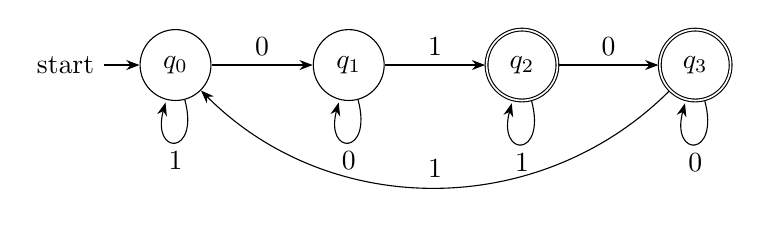
\begin{tikzpicture}[
    >=Stealth,
    node distance=2.2cm,
    on grid,
    auto,
    every state/.style={
        draw,
        circle,
        minimum size=0.9cm
    }
]

% states
\node[state, initial] (q0) {$q_0$};
\node[state, right=of q0] (q1) {$q_1$};
\node[state, accepting, right=of q1] (q2) {$q_2$};
\node[state, accepting, right=of q2] (q3) {$q_3$};
% transitions
\path[->]
(q0) edge node {$0$} (q1)
(q1) edge node {$1$} (q2)
(q2) edge node {$0$} (q3)

(q0) edge[loop below] node {$1$} ()
(q1) edge[loop below] node {$0$} ()
(q2) edge[loop below] node {$1$} ()
(q3) edge[loop below] node {$0$} ()

(q3) edge[bend left=45] node[above] {$1$} (q0);
\end{tikzpicture}
\end{center}
\subsubsection{NFA}
\[
NFA = (Q, \Sigma, \delta, q_0, F)
\]
\begin{flalign*}
Q &= \{q_0, q_1, q_2\cdots\} & \\
\Sigma &= \{a, b, c\cdots\} & \\
\delta &: Q \times \Sigma \to 2^Q = \{S | S \subseteq Q\} & \\
q_0 &\in Q(\text{一个开始状态}) & \\
F &\subseteq Q(\text{一个或多个接受状态}) &
\end{flalign*}
显而易见，每个DFA都是一个NFA。
\theorem{}{每一个NFA都可以转换成一个等价的DFA。}
\begin{proof}
设NFA为$N=(Q, \Sigma, \delta, q_0, F)$，我们构造一个DFA$D=(Q', \Sigma, \delta', q_0', F')$，其中：
\begin{itemize}
\item $Q' = 2^Q$，即DFA的状态集合是NFA状态集合的幂集。
\item $q_0' = \{q_0\}$，DFA的初始状态是NFA的初始状态的集合。
\item 对于每个状态集合$S \subseteq Q$和输入符号$a \in \Sigma$，定义$\delta'(S, a) = \bigcup_{q \in S} \delta(q, a)$，即DFA在状态集合$S$上输入符号$a$时转移到所有NFA状态$q$在输入符号$a$时转移的状态集合的并集。
\item $F' = \{S \subseteq Q | S \cap F \neq \emptyset\}$，DFA的接受状态集合是所有包含至少一个NFA接受状态的状态集合。
\end{itemize}
通过上述构造，我们可以证明DFA $D$接受的语言与NFA $N$接受的语言相同。对于任意输入字符串，DFA $D$在状态集合上进行转移，而NFA $N$在单个状态上进行转移。由于DFA $D$的状态集合包含了NFA $N$的所有可能状态，因此DFA $D$能够模拟NFA $N$的行为，并且接受相同的语言。
\end{proof}
NFA转化DFA例子：
这是一个NFA，接受语言$L$，其中
\[L=\{w \in \{0,1\}^* \mid w \text{ 以 }01\text{ 结尾}\}\]
\begin{center}
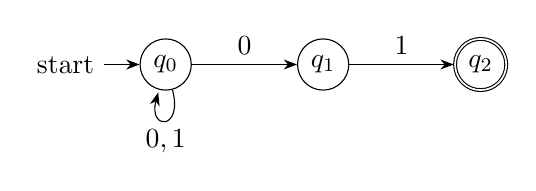
\begin{tikzpicture}[
    >=Stealth,
    node distance=2cm,
    on grid,
    auto,
    every state/.style={
        draw,
        circle,
        minimum size=0.65cm,
        inner sep=1pt
    }
]

\node[state, initial, initial text=start] (q0) {$q_0$};
\node[state, right=of q0] (q1) {$q_1$};
\node[state, accepting, right=of q1] (q2) {$q_2$};
\path[->]
(q0) edge node[above] {$0$} (q1)
(q1) edge node[above] {$1$} (q2)
(q0) edge[loop below] node {$0,1$} ();
\end{tikzpicture}
\end{center}

列出DFA所有可能状态集合：
\[
\begin{array}{|c|c|c|}
\hline
                     & 0                & 1                \\
\hline
\varnothing          & \varnothing      & \varnothing      \\
\hline
\{q_0\}              & \{q_0, q_1\}     & \{q_0\}          \\
\hline
\{q_1\}              & \varnothing      & \{q_2\}          \\
\hline
\{q_2\}              & \varnothing      & \varnothing      \\
\hline
\{q_0, q_1\}         & \{q_0, q_1\}     & \{q_0, q_2\}     \\
\hline
\{q_0, q_2\}         & \{q_0, q_1\}     & \{q_0\}          \\
\hline
\{q_1, q_2\}         & \varnothing      & \{q_2\}          \\
\hline
\{q_0, q_1, q_2\}    & \{q_0, q_1\}     & \{q_0, q_2\}     \\
\hline
\end{array}
\]
删除含有$\varnothing$的状态，删除不可达的状态，得到DFA状态转移表：
\[
\begin{array}{|c|c|c|c|}
\hline
\text{状态}            & 0                & 1                & \text{备注}      \\
\hline
A=\{q_0\}              & B                & A                & \text{初态}       \\
\hline
B=\{q_0, q_1\}         & B                & C                &                   \\
\hline
C=\{q_0, q_2\}         & B                & A                & \text{接受状态}    \\
\hline
\end{array}
\]
其中初态和NFA的初态相同，接受状态是所有包含NFA接受状态的状态集合。
构造DFA状态转移图：
\begin{center}
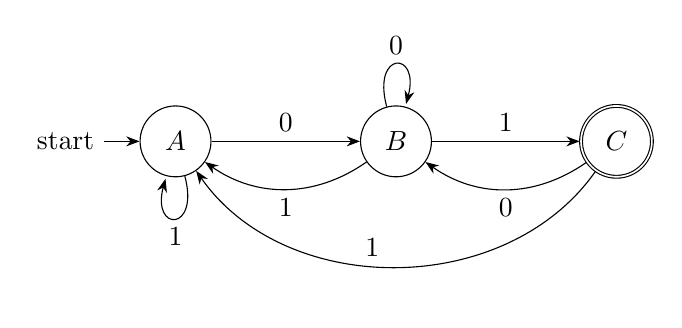
\begin{tikzpicture}[
    >=Stealth,
    node distance=2.8cm,
    on grid,
    auto,
    every state/.style={
        draw,
        circle,
        minimum size=0.9cm
    }
]

% states
\node[state, initial] (A) {$A$};
\node[state, right=of A] (B) {$B$};
\node[state, accepting, right=of B] (C) {$C$};
% transitions
\path[->]
(A) edge node[above] {$0$} (B)
(B) edge node[above] {$1$} (C)

(C) edge[bend left=35] node[below] {$0$} (B)
(B) edge[bend left=35] node[below] {$1$} (A)

(A) edge[loop below] node {$1$} ()
(B) edge[loop above] node {$0$} ()

(C) edge[bend left=55] node[above, pos=0.55] {$1$} (A);
\end{tikzpicture}
\end{center}


\subsubsection{$\varepsilon$-NFA}
\[
\varepsilon\text{-NFA} = (Q, \Sigma, \delta, q_0, F)
\]
\begin{flalign*}
Q &= \{q_0, q_1, q_2\cdots\} & \\
\Sigma &= \{a, b, c\cdots\} & \\
\delta &: Q \times (\Sigma \cup \{\varepsilon\}) \to 2^Q & \\
q_0 &\in Q(\text{一个开始状态}) & \\
F &\subseteq Q(\text{一个或多个接受状态}) &
\end{flalign*}
此后除非特别申明，不再明确区分$\varepsilon$-NFA和NFA, 而是都称为NFA。
\subsubsection{状态的$\varepsilon$-闭包}
状态q的$\varepsilon$-闭包是指从状态q出发，通过$\varepsilon$转移可以到达的所有状态的集合，记为$ECLOSE(q)$。
递归定义如下：
\begin{itemize}
\item $q \in ECLOSE(q)$
\item $\forall p \in ECLOSE(q), \forall r \in \delta(p, \varepsilon), r \in ECLOSE(q)$
\end{itemize}
相应状态集的$\varepsilon$-闭包定义为
\[
ECLOSE(S) = \bigcup_{q \in S} ECLOSE(q)
\]
\subsubsection{扩展转移函数}
对于NFA $N=(Q, \Sigma, \delta, q_0, F)$，定义扩展转移函数$\hat{\delta}: Q \times \Sigma^* \to 2^Q$如下：
\begin{itemize}
\item $\hat{\delta}(q, \varepsilon) = ECLOSE(q)$
\item $\hat{\delta}(q, wa) = \bigcup_{p \in \hat{\delta}(q, w)} ECLOSE(\delta(p, a))$，其中$w \in \Sigma^*$，$a \in \Sigma$。
即是$\hat{\delta}(q, w)$的可达状态集合
\end{itemize}
\theorem{}{每一个$\varepsilon$-NFA都可以转换成一个等价的DFA。}
\begin{proof}
设$\varepsilon$-NFA为$N=(Q, \Sigma, \delta, q_0, F)$，我们构造一个DFA$D=(Q', \Sigma, \delta', q_0', F')$，其中：
\begin{itemize}
\item $Q' = 2^Q$，即DFA的状态集合是NFA状态集合的幂集。
\item $q_0' = ECLOSE(q_0)$，DFA的初始状态是NFA的初始状态的$\varepsilon$-闭包。
\item 对于每个状态集合$S \subseteq Q$和输入符号$a \in \Sigma$，定义$\delta'(S, a) = \bigcup_{q \in S} ECLOSE(\delta(q, a))$，即DFA在状态集合$S$上输入符号$a$时转移到所有NFA状态$q$在输入符号$a$时转移的状态集合的$\varepsilon$-闭包的并集。
\item $F' = \{S \subseteq Q | S \cap F \neq \emptyset\}$，DFA的接受状态集合是所有包含至少一个NFA接受状态的状态集合。
\end{itemize}
\end{proof}
$\varepsilon$-NFA到DFA的转换例子：
这是一个$\varepsilon$-NFA，接受语言$L$，其中
\[L=\{w \in \{0,1\}^* \mid w \text{ 以 }01\text{ 结尾}\}\]
\begin{center}
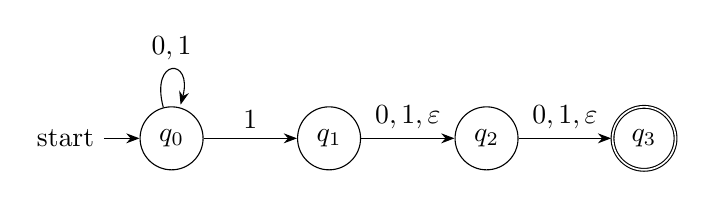
\begin{tikzpicture}[
    >=Stealth,
    node distance=2cm,
    on grid,
    auto,
    every state/.style={
        draw,
        circle,
        minimum size=0.8cm
    }
]

% states
\node[state, initial, initial text=start] (q0) {$q_0$};
\node[state, right=of q0] (q1) {$q_1$};
\node[state, right=of q1] (q2) {$q_2$};
\node[state, accepting, right=of q2] (q3) {$q_3$};
% transitions
\path[->]
(q0) edge[loop above] node {$0,1$} ()
(q0) edge node[above] {$1$} (q1)
(q1) edge node[above] {$0,1,\varepsilon$} (q2)
(q2) edge node[above] {$0,1,\varepsilon$} (q3);
\end{tikzpicture}
\end{center}
列出DFA所有可能状态集合：
\[
\begin{array}{|c|c|c|}
\hline
                                & 0                      & 1                      \\
\hline
\varnothing                     & \varnothing            & \varnothing            \\
\hline
\{q_0\}                         & \{q_0\}                & \{q_0, q_1, q_2, q_3\} \\
\hline
\{q_1\}                         & \{q_2, q_3\}           & \{q_2, q_3\}           \\
\hline
\{q_2\}                         & \{q_3\}                & \{q_3\}                \\
\hline
\{q_3\}                         & \varnothing            & \varnothing            \\
\hline
\{q_0, q_1\}                    & \{q_0, q_2, q_3\}      & \{q_0, q_1, q_2, q_3\} \\
\hline
\{q_0, q_2\}                    & \{q_0, q_3\}           & \{q_0, q_1, q_2, q_3\} \\
\hline
\{q_0, q_3\}                    & \{q_0\}                & \{q_0, q_1, q_2, q_3\} \\
\hline
\{q_1, q_2\}                    & \{q_2, q_3\}           & \{q_2, q_3\}           \\
\hline
\{q_1, q_3\}                    & \{q_2, q_3\}           & \{q_2, q_3\}           \\
\hline
\{q_2, q_3\}                    & \{q_3\}                & \{q_3\}                \\
\hline
\{q_0, q_1, q_2\}               & \{q_0, q_2, q_3\}      & \{q_0, q_1, q_2, q_3\} \\
\hline
\{q_0, q_1, q_3\}               & \{q_0, q_2, q_3\}      & \{q_0, q_1, q_2, q_3\} \\
\hline
\{q_0, q_2, q_3\}               & \{q_0, q_3\}           & \{q_0, q_1, q_2, q_3\} \\
\hline
\{q_1, q_2, q_3\}               & \{q_2, q_3\}           & \{q_2, q_3\}           \\
\hline
\{q_0, q_1, q_2, q_3\}          & \{q_0, q_2, q_3\}      & \{q_0, q_1, q_2, q_3\} \\
\hline
\end{array}
\]
删除含有$\varnothing$的状态，删除不可达的状态，得到DFA状态转移表：
\[
\begin{array}{|c|c|c|c|}
\hline
\text{状态}                        & 0                & 1                & \text{备注}      \\
\hline
A=\{q_0\}                          & A                & B                & \text{初态}       \\
\hline
B=\{q_0, q_1, q_2, q_3\}           & C                & B                & \text{接受状态}    \\
\hline
C=\{q_0, q_2, q_3\}                & D                & B                & \text{接受状态}    \\
\hline
D=\{q_0, q_3\}                     & A                & B                & \text{接受状态}    \\
\hline
\end{array}
\]
构造DFA状态转移图：
\begin{center}
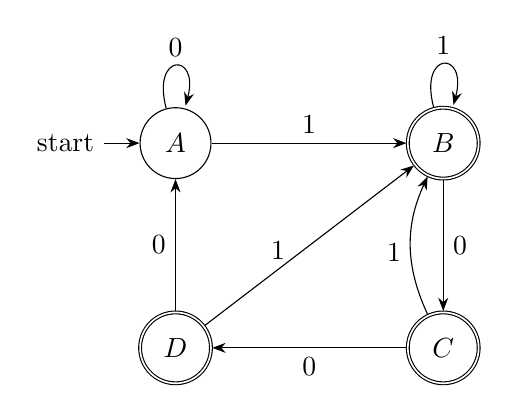
\begin{tikzpicture}[
    >=Stealth,
    node distance=2.6cm and 3.4cm,
    on grid,
    auto,
    every state/.style={
        draw,
        circle,
        minimum size=0.9cm
    }
]

% states
\node[state, initial] (A) {$A$};
\node[state, accepting, right=of A] (B) {$B$};
\node[state, accepting, below=of B] (C) {$C$};
\node[state, accepting, below=of A] (D) {$D$};
% transitions
\path[->]
% square edges
(A) edge node[above] {$1$} (B)
(B) edge node[right] {$0$} (C)
(C) edge node[below] {$0$} (D)
(D) edge node[left] {$0$} (A)

% loops
(A) edge[loop above] node {$0$} ()
(B) edge[loop above] node {$1$} ()

% C -> B, slightly curved to avoid B -> C
(C) edge[bend left=25] node[left, pos=0.45] {$1$} (B)

% D -> B, route outside
(D) edge node[pos=0.35, above] {$1$} (B);
\end{tikzpicture}
\end{center}
例题：设计一个$\varepsilon$-NFA，接受语言$L$，其中
\[L=\{w | w \in \{a,b,c\}^*\wedge w\text{的前$5$位至少有一个子串bac} \wedge 
w\text{的后$5$位至少有一个子串acb}\}\]
可以考虑到$xxbacbxx$和$xxbacxx+xxacbxx$的形式

但是还需要足够attention发现$acbac$的形式
\begin{center}
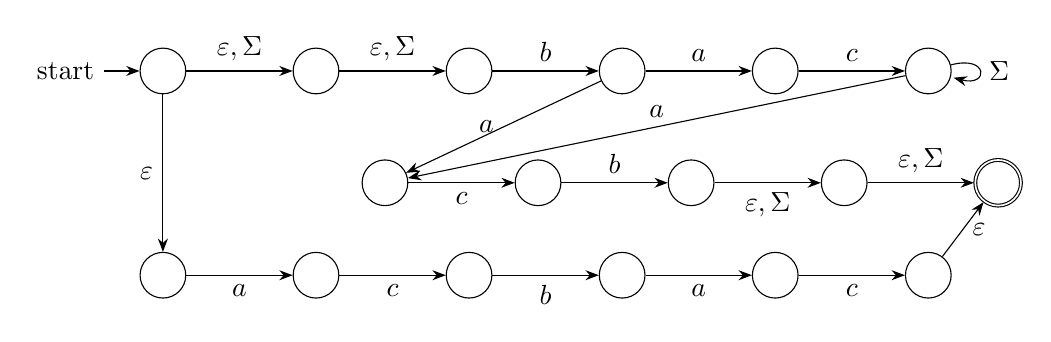
\begin{tikzpicture}[
    >=Stealth,
    node distance=1.25cm and 1.35cm,
    auto,
    every state/.style={
        draw,
        circle,
        minimum size=0.58cm,
        inner sep=1pt
    }
]

% upper branch
\node[state, initial] (q0) {};
\node[state, right=of q0] (q1) {};
\node[state, right=of q1] (q2) {};
\node[state, right=of q2] (q3) {};
\node[state, right=of q3] (q4) {};
\node[state, right=of q4] (q5) {};

% middle branch
\node[state, below right=1.0cm and 2.4cm of q0] (p0) {};
\node[state, right=of p0] (p1) {};
\node[state, right=of p1] (p2) {};
\node[state, right=of p2] (p3) {};
\node[state, accepting, right=of p3] (f) {};

% lower branch
\node[state, below=2.0cm of q0] (r0) {};
\node[state, right=of r0] (r1) {};
\node[state, right=of r1] (r2) {};
\node[state, right=of r2] (r3) {};
\node[state, right=of r3] (r4) {};
\node[state, right=of r4] (r5) {};
% transitions
\path[->]
% upper branch
(q0) edge node[above] {$\varepsilon,\Sigma$} (q1)
(q1) edge node[above] {$\varepsilon,\Sigma$} (q2)
(q2) edge node[above] {$b$} (q3)
(q3) edge node[above] {$a$} (q4)
(q4) edge node[above] {$c$} (q5)
(q5) edge[loop right] node {$\Sigma$} ()

% diagonals to middle branch
(q3) edge node[left] {$a$} (p0)
(q5) edge node[above] {$a$} (p0)

% middle branch
(p0) edge node[below] {$c$} (p1)
(p1) edge node[above] {$b$} (p2)
(p2) edge node[below] {$\varepsilon,\Sigma$} (p3)
(p3) edge node[above] {$\varepsilon,\Sigma$} (f)

% lower branch
(q0) edge node[left] {$\varepsilon$} (r0)
(r0) edge node[below] {$a$} (r1)
(r1) edge node[below] {$c$} (r2)
(r2) edge node[below] {$b$} (r3)
(r3) edge node[below] {$a$} (r4)
(r4) edge node[below] {$c$} (r5)
(r5) edge node[right] {$\varepsilon$} (f);
\end{tikzpicture}
\end{center}
\subsubsection{正则表达式}
有穷自动机接受的语言即是正则语言
正则语言可以通过代数式表示或产生

正则语言(Regular Language, RL)
的3种代数运算
\begin{itemize}
    \item 并(union) $L \bigcup M = \{w | w \in L \bigvee w \in M\}$
    \item 串接(concatenation) $L \cdot M = \{w | w = xy, x \in L, y \in M\}$
    \item 克林闭包(Kleene star) $L^* = \{w | w = x_1 x_2 \cdots x_k, k \geq 0, x_i \in L\}$   
\end{itemize}
注意：$L^0 = \{\varepsilon\}, \emptyset^* =\emptyset^0 = \{\varepsilon\}, \emptyset^n = \emptyset$

$L^+ = L^* - \{\varepsilon\}$

正则语言的正则运算结果都是正则语言，$\emptyset$也是正则语言。
例1：设计正则表达式$E$使得$L(E) = \{0, 1\}^*$
\[E = (0 + 1)^*\]
例2：设计正则表达式$E$使得$L(E) = \{w | w\text{的长度为$2$且第二个字符为$1$}\}$
\[E = (0+1)1\]

\theorem{}{$L$是一个正则表达式$R$表示的语言，则存在一个$\varepsilon$-NFA $M$
使得$L(M) = L(R) = L$}
\begin{proof}
    结构归纳法构造满足以下条件的等价$\varepsilon$-NFA $M$
\begin{itemize}
    \item 有一个初态和终态
    \item 没有弧进入初态
    \item 没有弧离开终态
\end{itemize}
Thompson构造法：
\begin{itemize}
    \item 对于$\varepsilon$，构造：
    \[
    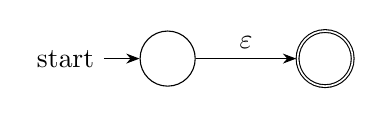
\begin{tikzpicture}[
        >=Stealth,
        node distance=2cm,
        on grid,
        auto,
        every state/.style={draw, circle, minimum size=0.7cm}
    ]
        \node[state, initial] (s) {};
        \node[state, accepting, right=of s] (f) {};
        \path[->]
        (s) edge node[above] {$\varepsilon$} (f);
\end{tikzpicture}
    \]

    \item 对于$\emptyset$，构造：
    \[
    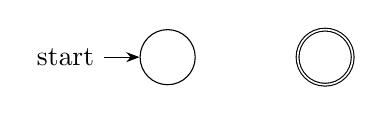
\begin{tikzpicture}[
        >=Stealth,
        node distance=2cm,
        on grid,
        auto,
        every state/.style={draw, circle, minimum size=0.7cm}
    ]
        \node[state, initial] (s) {};
\node[state, accepting, right=of s] (f) {};
    \end{tikzpicture}
    \]

    \item 对于$a$，构造：
    \[
    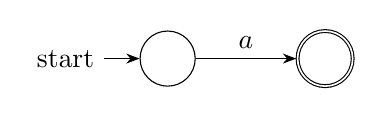
\begin{tikzpicture}[
        >=Stealth,
        node distance=2cm,
        on grid,
        auto,
        every state/.style={draw, circle, minimum size=0.7cm}
    ]
        \node[state, initial] (s) {};
\node[state, accepting, right=of s] (f) {};
        \path[->]
        (s) edge node[above] {$a$} (f);
\end{tikzpicture}
    \]

    \item 对于$E + F$，构造：
    \[
    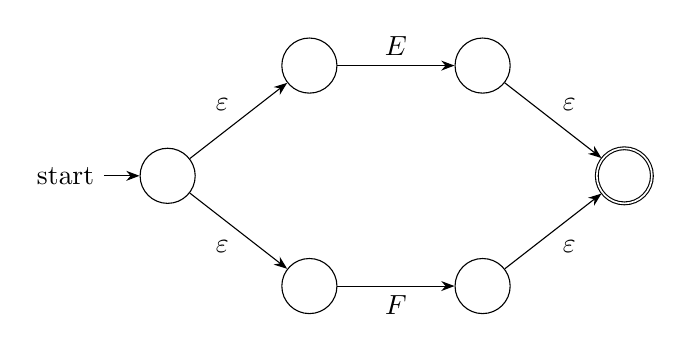
\begin{tikzpicture}[
        >=Stealth,
        node distance=1.4cm and 1.8cm,
        on grid,
        auto,
        every state/.style={draw, circle, minimum size=0.7cm}
    ]
        \node[state, initial] (s) {};
\node[state, above right=of s] (e1) {};
        \node[state, right=2.2cm of e1] (e2) {};
        \node[state, below right=of s] (f1) {};
\node[state, right=2.2cm of f1] (f2) {};
        \node[state, accepting, below right=of e2] (t) {};
\path[->]
        (s) edge node[above left] {$\varepsilon$} (e1)
        (s) edge node[below left] {$\varepsilon$} (f1)
        (e1) edge node[above] {$E$} (e2)
        (f1) edge node[below] {$F$} (f2)
        (e2) edge node[above right] {$\varepsilon$} (t)
        (f2) edge node[below right] {$\varepsilon$} (t);
\end{tikzpicture}
    \]

    \item 对于$EF$，构造：
    \[
    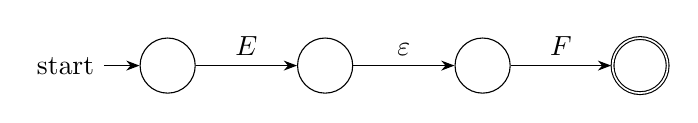
\begin{tikzpicture}[
        >=Stealth,
        node distance=2cm,
        on grid,
        auto,
        every state/.style={draw, circle, minimum size=0.7cm}
    ]
        \node[state, initial] (e1) {};
\node[state, right=of e1] (e2) {};
        \node[state, right=of e2] (f1) {};
        \node[state, accepting, right=of f1] (f2) {};
\path[->]
        (e1) edge node[above] {$E$} (e2)
        (e2) edge node[above] {$\varepsilon$} (f1)
        (f1) edge node[above] {$F$} (f2);
\end{tikzpicture}
    \]

    \item 对于$E^*$，构造：
    \[
    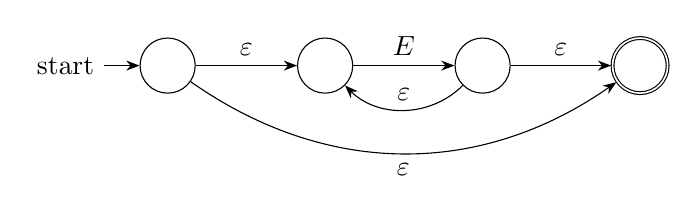
\begin{tikzpicture}[
        >=Stealth,
        node distance=2cm,
        on grid,
        auto,
        every state/.style={draw, circle, minimum size=0.7cm}
    ]
        \node[state, initial] (s) {};
\node[state, right=of s] (e1) {};
        \node[state, right=of e1] (e2) {};
        \node[state, accepting, right=of e2] (t) {};
\path[->]
        (s) edge node[above] {$\varepsilon$} (e1)
        (e1) edge node[above] {$E$} (e2)
        (e2) edge node[above] {$\varepsilon$} (t)

        (s) edge[bend right=35] node[below] {$\varepsilon$} (t)
        (e2) edge[bend left=45] node[above] {$\varepsilon$} (e1);
\end{tikzpicture}
    \]
\end{itemize}
\end{proof}

\theorem{}{$L$是某个$DFA D$表示的语言，则存在一个正则表达式$R$使得$L(R) = L(D) = L$}
\begin{proof}
Kleene构造法：
\begin{itemize}
    \item $D$的状态集用$\{1, 2, \dots, n\}$表示，其中初态为$1$
    \item 对$\forall 1 \leq i, j \leq n, 0 \leq k \leq n $，定义
    $R_{i,j}^k$表示从状态$i$到状态$j$且不经过状态$\{1, 2, \dots, k\}$之外的状态的路径上的标签组成的正则表达式
    \item $k = 0$时候
    \[
        R_{i,j}^0 = \begin{cases}
            \varepsilon, &i = j \text{且无自环}\\
            \varepsilon \mid a, &i = j \text{有自环}a\\
            \emptyset, &i \neq j \text{且无弧}i \to j\\
            a_1 \mid a_2 \mid \cdots \mid a_m, &i \neq j \text{有弧}i \to j\text{且有弧}a_1, a_2, \dots, a_m
        \end{cases}
    \]
    \item $k > 0$时候
    \[
        R_{i,j}^k = R_{i,j}^{k-1} \mid R_{i,k}^{k-1} (R_{k,k}^{k-1})^* R_{k,j}^{k-1}
    \]
    \item $L = \bigcup_{j \in F} R_{1,j}^n$
\end{itemize}
状态消除法：
\begin{itemize}
    \item 利用$\varepsilon$增加新的初态和新的接受态
    \item 对于$a$个入度，$b$个出度的节点，删除节点并添加$a*b$个弧
    \item 重复直到删除所有非初态非接受态的节点
\end{itemize}
\end{proof}

\theorem{Pumping Lemma for Regular Languages}{
    如果$L$是一个正则语言，则存在一个整数$p \geq 1$使得对于任意字符串$s \in L$且$|s| \geq p$，可以将$s$分解为三个部分$s = xyz$，满足以下条件：
    \begin{itemize}
        \item $|y| > 0$（即$y$不为空）
        \item $|xy| \leq p$（即$xy$的长度不超过$p$）
        \item 对于所有$i \geq 0$，字符串$xy^iz$也属于$L$
    \end{itemize}
}
\begin{proof}
    设$L$是DFA D的语言，取$n = |Q|$易证。
\end{proof}

正则语言对于下列运算封闭：
\begin{itemize}
    \item 并(union)
    \item 串接(concatenation)
    \item 克林闭包(Kleene star)
    \item 交(intersection)
    \item 补(complement)
    \item 反转(reverse)
    \item 同态(homomorphism)
    \item 逆同态(inverse homomorphism)
    \item 差(difference)
\end{itemize}
在正则语言的证伪中，泵引理的使用范围可推广到封闭运算结果

\theorem{}{具有$n$个状态的有穷自动机$M$接受的集合$S$；
    \begin{itemize}
        \item $S$是非空的等价$M$接受某个长度小于$n$的串
        \item $S$是无穷的等价$M$接受某个$n \leq |s| < 2n$的串$s$
    \end{itemize}
}
填表法最小化DFA：
\begin{itemize}
    \item 对于终态和非终态填区别
    \item 扫描所有剩下的状态对$(p, q)$，对其遍历$\sigma$，如果结果$(e, f)$已经区别，则区别。
    \item 重复扫描直到一次扫描没有更新
    \item 合并所有未区别的状态，合并状态时合并所有入度和出度和环
\end{itemize}
\subsection{上下文有关文法}
\subsubsection{CFG}
\[
CFG = (V, \Sigma, P, S)
\]
\begin{flalign*}
V & \text{是一个有限的非终结符集合} &\\
\Sigma & \text{是一个有限的终结符集合，且 } V \cap \Sigma = \emptyset &\\
P & \text{是一个有限的产生式集合，每个产生式的形式为 } A \to \alpha \text{，其中 } A \in V \text{ 且 } \alpha \in (V \cup \Sigma)^* &\\
S & \in V \text{ 是开始符号} &
\end{flalign*}
正向执行CFG称为派生，反之为归约

其中派生有最左和最右派生
\subsubsection{上下文无关语言}
上下文无关文法$G = (V, \Sigma, P, S)$的语言为
\[
    L(G) = \{w | w \in \Sigma^*, S\xrightarrow[G]{*} w \}
\]
\theorem{}{每个非空的CFL都能被一个不带无用符号的CFG定义}
\begin{itemize}
    \item 消除非产生的$(\xrightarrow[]{}\text{右边不能全部转化为}\Sigma)$
    \item 消除非可达的$($不能从$S$生成$)$
\end{itemize}
\theorem{}{任何$CFG-G$，都存在一个不带无用符号和$\varepsilon-$产生式的$CFG-G_1$
使得$L(G_1) = L(G) - {\varepsilon}$}

\subsubsection{乔姆斯基范式(CNF)}
\theorem{}{每个不带$\varepsilon$的CFL都可以由这样的CFG $G$定义，G中每个产生式的形式都为 $A \to BC$ 或 $A \to a$，其中$A, B, C$是变元，$a$是终结符。}
CFG转为CNF的方法：
\begin{itemize}
    \item 设文法不带无用符号、$\varepsilon$-产生式和单元产生式（任何文法都可以化简成这种形式）。
    \item 二叉化：考虑文法每个形式为 $A\rightarrow X_{1}X_{2}\cdot\cdot\cdot X_{m}(m\ge2)$ 的产生式，将变元串分解为二叉形式。
    \item 引入变量：处理含有多个符号的产生式时，将其中的终结符用新的变元进行替换。
\end{itemize}

\subsubsection{格雷巴赫范式(GNF)}
\theorem{}{每个不带$\varepsilon$的CFL都可以由这样的CFG $G$定义，G中每个产生式的形式都为 $A \to a\alpha$，其中$A$是变元，$a$是终结符，$\alpha$是零或多个变元的串。}
\begin{itemize}
    \item GNF的每个产生式都会引入一个终结符。
    \item 长度为$n$的串的派生恰好是$n$步。
\end{itemize}

\subsubsection{下推自动机}
下推自动机$PDA/NPDA = (Q, \Sigma , \Gamma , \delta , q_0 , Z_0 , F)$
\begin{flalign*}
Q & \text{有穷状态集} &\\
\Sigma &\text{有穷输入符号} &\\
\Gamma &\text{有穷堆栈符号} &\\
\delta &\text{转移函数} &\\
q_0 &\in Q \text{一个开始状态} &\\
Z_0 &\in \Gamma \text{一个开始堆栈符号} &\\
F &\subseteq Q \text{终态集合} &
\end{flalign*}

\subsection{短语文法}
\end{document}